To test whether the binary per-device setup is the binding constraint,
a single BiGRU + TF-Aug is trained on all 12 devices simultaneously
(12-class softmax). The model has access to the full \nWindowedSamples-sample windowed
DGT cache, compared to the $\approx$52 samples available to each binary
classifier in trial\_1.

\begin{table}[htbp]
\centering
\caption{Multi-class BiGRU vs.\ binary LOTO (trial\_1, 5 seeds).}
\label{tab:multiclass}
\begin{tabular}{lcc}
\toprule
\textbf{Setting} & \textbf{Metric} & \textbf{Value} \\
\midrule
Binary LOTO (BiGRU)    & mean ADR  & \bigruLOTOadrMean \\
Multi-class (BiGRU)    & accuracy  & $\mcAccuracy \pm \mcAccuracyStd$ \\
Multi-class (BiGRU)    & macro F1  & $\mcMacroFone \pm \mcMacroFoneStd$ \\
Random baseline (1/12) & accuracy  & \mcRandomBaseline \\
\bottomrule
\end{tabular}
\end{table}

% figures/fig_mc_confusion and fig_mc_perclass not yet generated (run notebook 04 export cell)
%\begin{figure}[htbp]
%  \centering
%  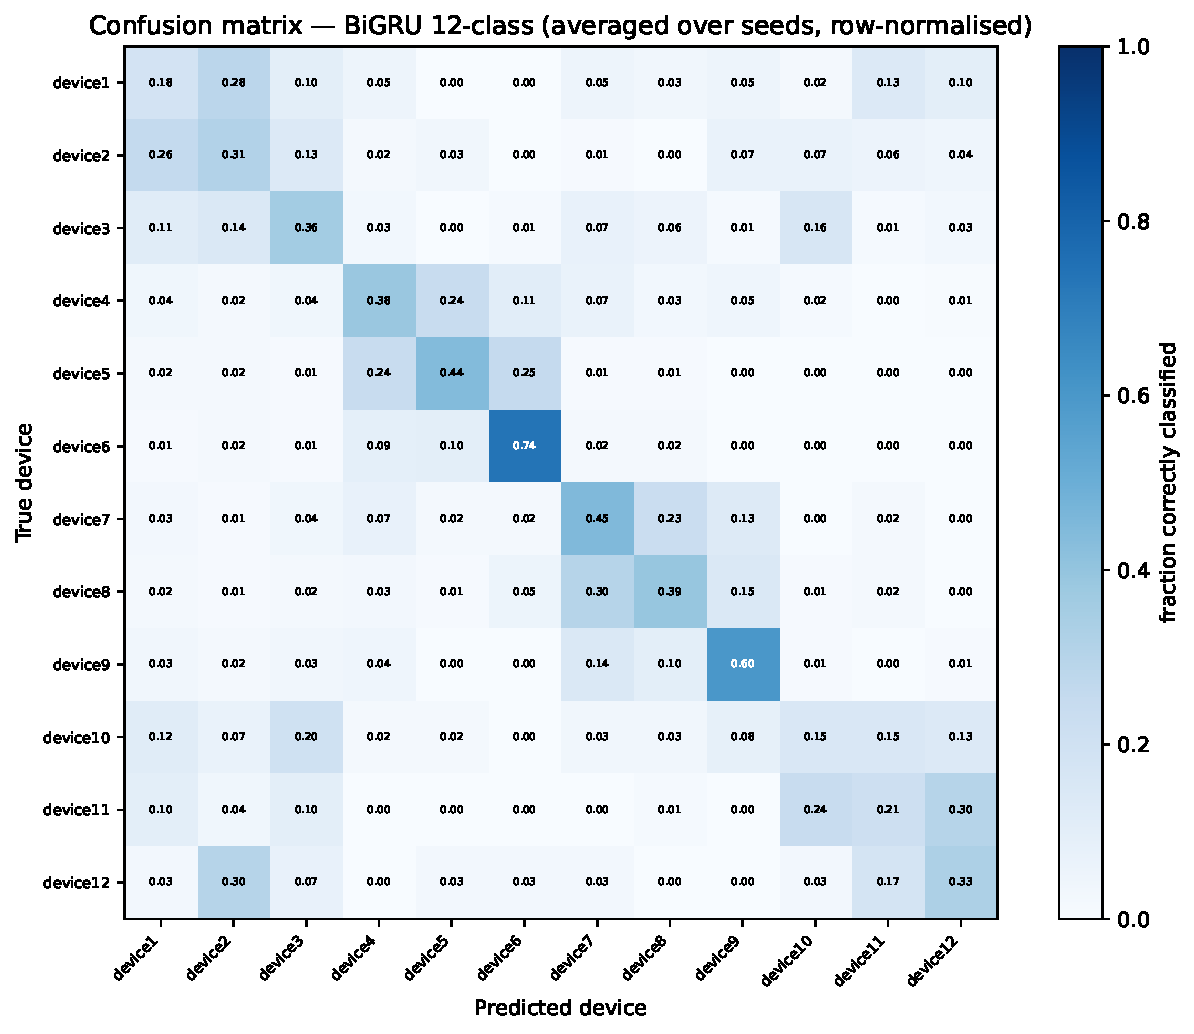
\includegraphics[width=\columnwidth]{figures/fig_mc_confusion}
%  \caption{Averaged confusion matrix (BiGRU, 12-class, 5 seeds).
%           Row-normalised; diagonal dominance indicates above-chance discrimination.}
%  \label{fig:mc_confusion}
%\end{figure}
%
%\begin{figure}[htbp]
%  \centering
%  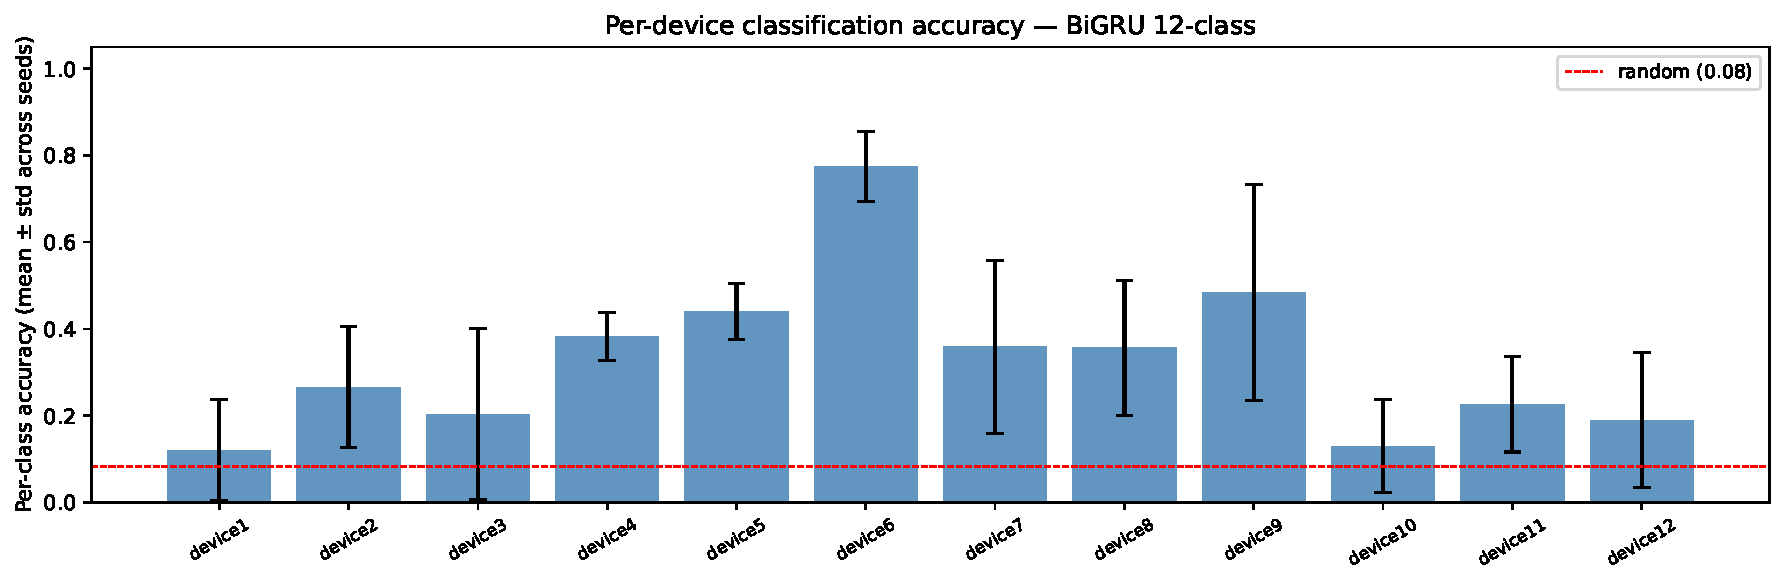
\includegraphics[width=\columnwidth]{figures/fig_mc_perclass}
%  \caption{Per-device classification accuracy (mean $\pm$ std, 5 seeds).
%           Devices with fewer raw transients (device10--12) show higher variance.}
%  \label{fig:mc_perclass}
%\end{figure}

The multi-class BiGRU achieves \mcAccuracy\% accuracy against a random baseline of
\mcRandomBaseline, confirming that the RF transient carries device-discriminating information across all 12 devices. In absolute terms this is lower than the binary LOTO ADR (\bigruLOTOadrMean), which reflects the harder 12-way classification task rather than a failure of the architecture. Devices 10--12, which have only 60 windowed samples each compared to 120--130 for devices 1--9, display the highest variance, reinforcing that per-device sample count is the primary performance driver.
